\chapter{Equipos de Bombeo}

\section{Introducción}
\subsection{Conceptos básicos}
\begin{definition}[Máquinas hidráulicas]
    Es un dispositivo que transforma la energía hidráulica a energía mecánica (motor hidráulico o turbinas)
\end{definition}
\begin{definition}[Bomba]
    Es un dispositivo que transforma energía mecánica a energía hidráulica
\end{definition}
% Generación de energía eléctrica
% \begin{equation}
%     Pot =\gamma\cdot Q\cdot H
% \end{equation}
% \begin{equation*}
%     Q =\int \bar{v}
% \end{equation*}
% Uso de turbinas hidráulicas para la producción de energía mecánica
% Turbina hidráulica y generador eléctrico acoplados por un eje
% Diferentes tipos de turbinas hidráulicas (Francis, Fixed pitch propeller turgo pelton kaplan)
% Funcionamiento de las turbinas
% PLanta con turbinas hidroeléctricas (oregon USA)
% Central hidroeléctrica
% Eficiencias de las turbinas
% Tipos de instalaciones hidroeléctrica
% Central hidroeléctrica de España

% La turbina es una máquina que transforma la energía cinética contenida en el fluido por velocidad o altura, en enetgía mecánica de movimiento de rotación. La energía disponible es la relación presentada arriba.
% \begin{equation}
%     E_T = \frac{1}{2}
% \end{equation}
% Rango de aplicación de las turbinas hidroeléctricas.
\subsection{Hidrodinámica}
Ecuaciones básicas, considerando el teorema del transporte de Reynolds
\begin{equation}
    \frac{Dn}{dt} = \frac{\partial }{\partial t} \int_{CV} \nu \rho \,dV + \int_{CS} \nu \rho \vec{V}\, d\vec{A}
\end{equation}
Primera ley de la termodinámica:
\begin{equation}
    \dot{Q} - \dot{W} = \frac{dE}{dt}
\end{equation}
Ecuación de continuidad
\begin{equation}
    m_1 - m_2 = \frac{\Delta m}{t}\implies m =\rho V
\end{equation}
entonces cuando el flujo es permanente e incompresible e isotérmico
\begin{align}
    m_1 = m_2&& pQ_1 = p_2Q_2
\end{align}
Ecuación de cantidad de movimiento, segunda ley de Newton:
\begin{equation}
    \sum \bar{F} = \sum \rho\cdot Q\cdot \bar{v}
\end{equation}
\begin{example}
    El móvil que se muestra tiene adjunto un álabe que desvía un chorro de agua en un ángulo de $60^{\circ}$. El chorro de agua sale de una tobera con una velocidad de 25 m/s y con área transversal de $5cm^2$, considere que el contacto con el álabe es tan poco que se puede despreciar la fuerza de roce con su superficie, de forma tal que el chorro sale con la misma velocidad y área pero deflectado el ángulo del álabe. Determine la fuerza F de sujeción necesaria para que el carro esté detenido. Considere que el fluido es agua con densidad de $1000kg/m^3$
\end{example}
\begin{figure}[h!]
\centering
  \includegraphics[width=0.5\textwidth]{eb1.png}
  \caption{Esquema del problema}
  \label{eb1}
\end{figure}
\textit{ Sol. }

El fluido ejercerá una fuerza horizontal y vertical sobre el carro, como la fuerza que nos solicita encontrar se halla en el eje x, se procede a aplicar la ecuación de conservación de la cantidad de movimiento en el eje horizontal:
\begin{equation*}
    \sum F_x = \sum F_{sx} + \sum F_{bx} = \frac{d}{dt} \int_{VC} \rho u\, dV +\int_{Sc} \rho u \vec{V}\, d\vec{A}
\end{equation*}
La selección del volumen de control es mostrado en la siguiente figura, la selección del volumen de control se hizo de forma tal que las superficies de control de entrada y salida estén perpendiculares al flujo
\begin{figure}[h!]
    \centering
      \includegraphics[width=0.5\textwidth]{eb2.png}
      \caption{Selección del volumen de control del problema planteado}
      \label{eb2}
    \end{figure}
En el eje de estudio no existan fuerzas volumétricas de forma tal que la ecuación que calcula la fuerza que le hace el móvil al fluido $Vc$ será:
\begin{equation*}
    F_x = F_{MF} = \frac{d}{dt} \int_{Vc}\rho u\, dV + \int_{SC1} \rho u \vec{V}\, d\vec{A} + \int_{SC2}\rho u \vec{V}\, d\vec{A}
\end{equation*}
Observe que el volumen de control no cambia con el tiempo, por lo que la primera integral es nula, aplicando la ecuación se tiene:
\begin{align*}
    &\frac{d}{dt}\int_{VC}\rho u\,dV = 0\\
    &\int_{SC1}\rho u \vec{V}\, d\vec{A} =-\rho V_1\left(V_1A\right)\\
    &\int_{SC2}\vec{V}\,d\vec{A} =\rho V_2\cos{\theta}\left(V_2A\right)
\end{align*}
Recordando que las velocidades $V_1=V_2=V$, se tiene que podemos expresarla como:
\begin{align*}
    &F_x = F_{M/F} =-\rho V(VA) +\rho V\cos{\theta}(VA)\\
    &F_x = F_{M/F} = \rho V^2A(\cos{\theta} - 1)
\end{align*}
Ahora por acción y reacción, se tiene que la fuerza que le hace el móvil al fluido es igual en magnitud y dirección, pero sentido contrario a la fuerza que el fluido le hace al móvil, es decir:
\begin{align*}
    &F_{F/M} = - F_{M/F}\\
    &F_{F/M} = -\rho V^2A\left(\cos{\theta} - 1 \right)
\end{align*}
Ahora haciendo balance de fuerzas horizontales sobre el móvil sabiendo que no existe aceleración, se tiene que:
\begin{align*}
    &F_{F/M} - F = 0\\
    &F = F_{F/M} = -\rho V^2A\left(\cos{\theta}- 1 \right)
\end{align*}
Sustituyendo los valores respectivos se tiene que $F=156.25N$

\subsection{Ejercicios de las ecuaciones fundamentales de la hidráulica}
\begin{problem}
    El agua entra en una tubería desde un recipiente de grandes dimensiones y después de abandonarla incide sobre un alabe deflector que desvía el chorro a $90^{\circ}$, según se muestra en la fig \ref{eb3}. si sobre el alabe deflector se desarrolla un empuje horizontal de 100kg. ¿Cuál es la potencia en caballos de vapor, desarrollada por la turbina si antes de la misma la presión es de $3kg/cm^2$?
\end{problem}
\begin{figure}[h!]
\centering
  \includegraphics[width=0.8\textwidth]{eb3.pdf}
  \caption{Problema 33 de Sotelo}
  \label{eb3}
\end{figure}
\textit{ Sol. }
El chorro de agua incide sobre el deflector es posible aplicar la ecuación siguiente:
\begin{equation*}
    F = 2\gamma A \frac{V^2}{2g}
\end{equation*}
Sabiendo que $F = 100kg$ entonces sustituyendo:
\begin{align*}
    &100 = 2(1000)(\pi\cdot 0.075^2)\frac{V^2}{2g}\\
    &V = \sqrt{\frac{100\cdot 19.62}{2 \cdot 100 \cdot \left(\pi \cdot (0.075)^2\right)}} = 7.4507 \frac{m}{s} \\
    &Q = A\cdot V = \left(7.4507\right)\left(\pi \cdot (0.075)^2\right) = 0.1316 \frac{m^3}{s}
\end{align*}
Aplicando la ecuación de la energía para determinar $H_{a,b}$
\begin{align*}
    &Z_1 = Z_2 = 0&& P_1 = P_2 = 0&&V_1 = V_2 = 0
\end{align*}
\begin{align*}
    &\frac{P_1}{\gamma} + Z_1 + \frac{V_1^2}{2g} = H_{a,b} + \frac{P_2}{\gamma} + Z_2 + \frac{V_2^2}{2g}\\
    &H_{a,b} =HQ\gamma = (30)(0.1316)(1000) = 39.48kg\cdot \frac{m}{s} = 52.64 C.V.
\end{align*}
\begin{problem}
    Una tubería horizontal de 6m de diámetro tiene un codo reductor que conduce al agua una tubería de 4m de diámetro, unida a $45^{\circ}$ de la anterior. la presión a la entrada del codo es de $10kg/cm^2$ y la velocidad de 15m/s. Determinar las componentes de la fuerza que han de soportar los anclajes del codo. Despreciar las pérdidas en el codo y el peso del líquido dentro del mismo.
\end{problem}
\begin{figure}[h!]
    \centering
    \includegraphics[width=0.8\textwidth]{eb4.pdf}
    \caption{Problema 37 de Sotelo}
    \label{eb4}
\end{figure}
\textit{ Sol. }
Aplicando la ecuación del gasto, obtenemos
\begin{equation*}
    Q_1 =15\left(\frac{\pi\cdot 6^2}{4} \right) = 424.11 \frac{m^3}{s}
\end{equation*}
Calculando $V_2$,  se aplica la ecuación de continuidad:
\begin{equation*}
    V_2 = \frac{A_1 \cdot V_1}{A_2}V_2 = \frac{\pi\left(\frac{D_1^2}{4}\right)}{\pi \cdot \left(\frac{D_2^2}{4}\right)}V_1 \implies V_2 = \frac{D_1^2}{D_2^2}V_1
\end{equation*}
Por lo tanto $V_2=33.75m/s$; aplicando la ecuación de la energía:
\begin{align*}
    &Z_1 + \frac{P_1}{\gamma} +\alpha_1\frac{V_1^2}{2g} = Z_2 + \frac{P_2}{\gamma} +\alpha_2\frac{V^2_2}{2g} + \frac{1}{2}hr\\
    &0 + \frac{100000}{1000} + \frac{1(15)^2}{19.62} = 0 + \frac{P_2}{\gamma} + \frac{1\left(33.75\right)^2}{19.62} + 0\\
    &\frac{P_2}{\gamma} = 52.421m \implies P_2 = 52421 \frac{kg}{m^2}
\end{align*}
Para el cálculo del empuje hidrodinámico en el eje x, aplicando la ecuación de impulso y cantidad de movimiento en la dirección “x”
\begin{equation*}
    F\rho ex + F\rho dx + Fcx + F\tau x= e\sum\left(QBV_x\right)
\end{equation*}
Sustituyendo valores
\begin{align*}
    &P_1A_1 - P_2A_2 \cos{45^{\circ}} - F\rho dx = eQ\left(B_2V_2 \cos{45^{\circ}} - B_1 V_1 \right)\\
    &F\rho dx = P_1A_1 - P_2A_2 \cos{45^{\circ}} - eQ\left(B_2V_2 \cos{45^{\circ}} - B_1V_1  \right)\\
    &F\rho = 100000\left(\frac{\pi(6)^2}{4}\right) - 52421 \left(\frac{\pi(4)^2}{4}\right)\cos{45^{\circ}} - 101.97(424.11) \left(33.75 \cos{45^{\circ}} - 15\right)\\
    &F\rho dx = 1969451.102kg = 1969.451 ton
\end{align*}
Cálculo de $F\rho dy$: Aplicando la ecuación de impulso cantidad y movimiento en $y$:
\begin{align*}
    &F\rho ey + F\rho dy + Fcy + F\tau y = e\sum \left(QBV_y\right)\\
    &- P_2A_2\sin{45^{\circ}} - F\rho dy = eQ\left(B_2V_2 \sin{45^{\circ}}\right)\\
    &F\rho dy = eQ\left(B_2V_2\sin{45^{\circ}} \right) + P_2A_2\sin{45^{\circ}}\\
    &F\rho dy = 52421\left(\frac{\pi(4)^2}{4}\right) \sin{45^{\circ}} + 101.97(424.11)\left(33.75 \cdot (\sin{45^{\circ}} )\right)\\
    &F\rho dx = 1,506,687.857kg = 1,506.687 ton
\end{align*}
\begin{problem}
    En la figura se tine un distribuidor de gasto, obtenga una ecuación que relacione $Q_2/Q_1$ con $\theta$. Además, calcule la fuerza F que obra sobre la placa, si $Q_2$ es el 80\% de Q. El conducto es cuadrado, de lado B.
\end{problem}
\begin{figure}[h!]
        \centering
          \includegraphics[width=0.8\textwidth]{eb5.pdf}
          \caption{Problema 39 de Sotelo}
          \label{eb5}
\end{figure}
\textit{ Sol. }

Por cantidad:
\begin{equation}
    Q=Q_1+Q_2
\end{equation}
Siendo la presión y las cotas las mismas en los puntos 0,1 y 2, las cargas de velocidades también deben ser las mismas:
\begin{equation}
    V_0=V_1=V_2=V
\end{equation}
Aplicando la ecuación del cambio de cantidad de movimiento en el eje x (paralelo a la placa)
\begin{align*}
    &\sum F_x=\rho Q_2V-\rho Q_1V-\rho QV\cos{\theta}\\
    &\rho Q_2 V-\rho Q_1V=\rho QV\cos{\theta}=0\\
    &Q_2-Q_1-Q\cos{\theta}=0\\
    &\left(Q-Q_1\right)*Q_1-Q\cos{\theta}=0\\
    &Q_1=Q\frac{\left(1-\cos{\theta}\right)}{2}\\
    &Q_1=Q\sin{\frac{\theta}{2}}\\
    &Q_2=Q\cos{\frac{\theta}{2}}\\
    &\frac{Q_2}{Q_1}=\cot{\frac{\theta}{2}}
\end{align*}
Según la ecuación cantidad de movimiento en el eje y
\begin{align*}
    &F=\rho Q\sin{\theta}\\
    &\rho=\frac{\gamma}{g}\implies Q=Vb\\
    &Q_2=0.8Q=\frac{Q\left(1+\cos{\theta}\right)}{2}\implies \sin{\theta}=0.8\\
    &F=\frac{\gamma}{g}\left(Vb\right)(V)(0.8)=0.8\frac{\gamma}{g}BV\quad\blacksquare
\end{align*}











\section{Ariete hidráulico}
El ariete hidráulico fue patentado en 1796, por Joseph Montgolfier (1749- 1810), consiste en una máquina que aprovecha únicamente la energía de un pequeño salto de agua para elevar parte de su caudal a una altura superior. A partir de su invención, el ariete hidráulico tuvo una amplia difusión por todo el mundo. Baste decir, a modo de ejemplo, que estuvo presente en las famosas fuentes del Taj Mahal en la India, o en el Ameer de Afganistán. Con el tiempo cayó en desuso, sobre todo debido al avance arrollador de la bomba centrífuga. En la actualidad asistimos a un renacer del interés acerca de este aparato, debido a que es tecnológicamente accesible. eficiente, ecológico y muy didáctico

\subsection{Funcionamiento}
El agua se acelera a lo largo del tubo de alimentación hasta alcanzar una velocidad suficiente como para que se cierre la válvula (A), Figura \ref{eb}. Entonces se crea una fuerte presión, al detenerse el agua bruscamente. Este golpe de presión abre la válvula (B) y hace pasar un pequeño chorro de agua al depósito (C), hasta que se equilibran las presiones. En ese momento, la gravedad abre la válvula (A) y se cierra la (B), repitiéndose de nuevo el ciclo. El agua, a cada golpe de aire hace fluir el agua, con continuidad, por la manguera de elevación.

El ritmo de golpes por segundo suele ser de uno o dos.
\begin{figure}[h!]
\centering
  \includegraphics[width=0.5\textwidth]{eb6.png}
  \caption{Ariete hidráulico}
  \label{eb6}
\end{figure}
Los fontaneros conocen muy bien el golpe de ariete; cuando se cierra bruscamente un circuito abierto de agua, toda la tubería se estremece y los manómetros enloquecen. A menudo se producen roturas por esta causa. El ariete hidráulico es una máquina que provoca continuos cierres bruscos de un circuito con agua en aceleración y que aprovecha las sobrepresiones para mandar parte del caudal a una gran altura.

\subsubsection{Altura de elevación (H)}
Como puede deducirse de la tabla anterior, a partir de 12 veces la altura (h), el rendimiento de los arietes disminuye en gran medida. Este detalle no nos ha de desalentar. Aunque sólo subamos a gran altura un 1\% del agua que pasa por nuestro ariete, este funciona las 8.760 horas del año, y sin combustible.

\subsubsection{Caudal elevado (Q)}
Depende del rendimiento (R), el caudal de alimentación (Q), el desnivel de trabajo (h) y la altura de elevación (H). La ecuación por la que se relacionan es la siguiente:
\begin{equation}
  q = r \cdot Q \cdot \frac{h}{H}
\end{equation}


\section{Bombas centrífugas}
\subsection{Funcionamiento, elementos constructivos y clasificación de bombas centrífugas}
La diferencia entre una Bomba y motobomba, son los impulsores.

Ecuación ideal o teórica:
\begin{equation}
    a?
\end{equation}
\begin{notation}
    \begin{itemize}
        \item $Q=$ Caudal o gasto
        \item $Q\gamma=$ peso del agua
        \item $D=$ Diámetro exterior del impulsor $D_1$
        \item $d=$ Diámetro exterior del impulsor $D_2$
        \item $b=$ ancho de boca del impulsor
        \item $U_1=$ Velocidad tangencial o periférica en el exterior del impulsor $u_1$
        \item $U=$ Velocidad periférica en el interior del impulsor $u_2$
        \item $V=$ Velocidad relativa del agua con respecto
        \item 
    \end{itemize}
\end{notation}
La velocidad se concentra en el aspa, de tal manera que en el centro, la velocidad del agua sea cero.

Hipótesis:
\begin{enumerate}
    \item Nulo espesor de los alabes que forman los conductores: Falso
    \item Nulas pérdidas energéticas (Fricción, en las tuberías y los pasos en las bombas): Falso
    \item Nula velocidad tangencial $V_t$ o de remolino en la entrada (no genera Fuerza dinámica en la entrada): Falso
    \item Entrada del agua tangencial al aspa o sea $v_r=V$: Falso.
\end{enumerate}

Presión Dinámica generada por la reacción en la salida del alabe del impulsor con la $V_{st}$
\begin{equation}
    P = R = \gamma Q \frac{v}{g}
\end{equation}
% FIGURA AQUI
Gasto en la entrada por el ojo del impulsor $Q=AV=\pi\cdot D\cdot b\cdot v_r$

Potencia hidráulica por fuerza dinámica, es igual a:
\begin{equation}
    Pot = \gamma Q \frac{v}{g} U_1
\end{equation}
\begin{notation}
    \begin{itemize}
        \item Pot= Fuerza por velocidad $P_dU$
    \end{itemize}
\end{notation}
Como



Sería la primera expresión de la ecuación para la bomba centrífuga, a partir del siguiente triángulo de velocidades del aspa:


Entonces del a figura, en la salida B:
\begin{align*}
    U_1 = V_{1t} + S&& V_t = U_1 - S\\
    V_1^2 = V_{1r}^2 + V_{1t}^2\\
    \tan{\beta_1} = \frac{V_{1t}}{S} &&
\end{align*}
\begin{align*}
    H = V_\frac{1t}{S}U_1 =
\end{align*}
Finalmente:
\begin{equation}
    H = \frac{U_1^2 - v_{14}^2 \csc^2{\beta_1} }{2g}
\end{equation}

Esta ecuación relaciona la velocidad angular en la felcha N (RPM)

Y si la velocidad radia nos representa el gastoQ, de las ecuaciones:
\begin{equation}
    U_1 = \frac{\pi D_1 N}{60}
\end{equation}
\begin{notation}
    \begin{itemize}
        \item Diámetro exterior del impulsor en metros m
        \item N= Velocidad angular en revoluciones por minuto RPM
    \end{itemize}
\end{notation}
Y el gasto:
\begin{equation}
    Q_1 = \pi D_1 b_1 v_{1r} \implies v_{1r} = \frac{Q_1}{\pi D b_1 }
\end{equation}
 Entonces la ecuación queda:
 \begin{equation}
    G = \frac{U_1^2}{2g} - \frac{Q^2 \csc^2{\beta_1} }{\left(\pi D b \right)^2 2g}
 \end{equation}
Simplificando en constantes
\begin{equation}
    H = H_0 - AQ^2
\end{equation}
% Ecuación de una parábola
\begin{example}
    Una bomba centrífuga de agua con 700 mm de diámetro exterior de impulsor gira a 1800 RPM. El agua entra en forma radial y sin pérdidas y se desprecia el espesor de los alabes, el ángulo entre la velocidad de salida tangencial U1 y la absoluta v1 es de $60^{\circ}$, la carga real que produce la bomba es de 22 m, encuentre la eficiencia hidráulica, si la velocidad absoluta de salida es de $v_1 = 6 m/s$
\end{example}
\textit{ Sol. }

Se tiene D=700mm, N=1700 RPM y una $H_{real}=15m$, la incógnita es la eficiencia en b $\nu_b$.
\begin{align*}
    &\nu = \frac{\text{Potencia Obtenida}}{\text{Potencia Suministrada}}\\
    &\text{Potencia}=FV\\
    &F =\rho Q\bar{V} = \frac{\gamma}{g}Q\bar{V}\\
    &H_{teorica} = \frac{V_1t}{g}  \cdot U_1\\
    &V_{1t} = v_1 \cdot \cos{60^{\circ}}\\
    &V_1 = 6m\text{ Velocidad absoluta de salida}\\
    &V_{1t} = 6 \cdot \cos{60^{\circ}} = 3m\\
    U_1 = \frac{\pi \cdot D \cdot N}{60} = \frac{\pi \cdot 0.7 \cdot  1700 }{60} = 62.3 \frac{m}{s}\\
    H_{teorica} = \frac{3 \cdot 62.3}{9.81} = 19.0545m\\
    \nu = \frac{15m}{19.0545} \cdot 100 = 78.72 \%\quad
\end{align*} 
\begin{example}
    Una bomba centrífuga tiene un impulsor con dimensiones r=75mm, r 1=150mm, b=50mm, b1=30mm, $\beta=300=\phi$, para una descarga de 12 lps y entrada sin choques, calcule:
    \begin{itemize}
        \item velocidad de rotación
        \item la carga
        \item el par o torque
        \item  la potencia, desprecie las pérdidas
    \end{itemize}
\textit{ Sol. }
\end{example}

Calculamos $V_{1r}$
\begin{align*}
    &Q = AV_r\\
    &V_r = \frac{Q}{\pi\left(D_1 \cdot b_1 \right)}\\
    &V_r = \frac{0.012\frac{m^3}{s}}{\pi\left(0.15m \cdot 0.05m  \right)} = 0.51 \frac{m}{s}\\
\end{align*}
Calculando V
\begin{align*}
    &\cos{60^{\circ}} \cdot  V = V_r\\
    &V = \frac{V_r}{\cos{60^{\circ}} }\\
    &V = \frac{2.9708}{\cos{60^{\circ}}}= 0.88 \frac{m}{s}
\end{align*}
Calculando $V_1$
\begin{align*}
    &\cos{\beta} \cdot v = V_1\\
    &V_1 = \cos{30^{\circ}} \cdot  5.9417 \frac{m}{s}\\
    &V_1 = 5.1456 \frac{m}{s}
\end{align*}
Obteniendo N:
\begin{equation*}
    V = \frac{\pi D \cdot N}{60} \implies N = \frac{60 \cdot V}{\pi \cdot D} = 655.1708 \approx 655 RPM\\
\end{equation*}
Conseguir $U_1$:
\begin{align*}
    U_1 = \frac{\pi \cdot D \cdot N }{60} = \frac{\pi \cdot 0.3 \cdot  655}{60} = 10.2887
\end{align*}
Despejando $V_{1r}$
\begin{align*}
    &Q = AV_{1r}\implies V_{1r}= \frac{Q}{\pi \left( D_1 \cdot b_1 \right)}\\
    &V_{1r}= \frac{0.07}{\pi\left( 0.3m \cdot 0.03m \right)} = 2.4757 \frac{m}{s}\\
    &V_1 \cdot \cos{60^{\circ}} = V_{1r}\implies V_1 = \frac{V_{1r}}{\cos{60^{\circ}}} = V_{1r}\\
    &V_1 = \frac{V_{1r}}{\cos{60^{\circ}}} = 4.9514 \frac{m}{s}
\end{align*}
Calculamos S:
\begin{align*}
    &\cos{30^{\circ}} \cdot  V_1 = S\\
    &S = 4.2880\\
    &V_1 = S +V_{1r}\implies V_{1t} = V_1 - S = 10.2887 \frac{m}{s} - 4.2880 \frac{m}{s} = 6.00007 \frac{m}{s}
\end{align*}
Calculando la carga H:
\begin{align*}
    H = \frac{V_{1t}}{g} = \frac{6.00007 \frac{m}{s} \cdot 10.2887 \frac{m}{s}}{9.81 \frac{m}{s^2}} = 6.2935m
\end{align*}
El torque es:
\begin{align*}
    &F = \gamma \cdot Q \cdot \frac{V_{1t}}{g} = 1000 \cdot 0.07 \cdot \frac{6.00007 }{9.81} = 42.8184m\\
    &Torque = F \cdot r_1 = 42.8184 \cdot 0.15 = 6.4227 \frac{Kg}{m}
\end{align*}
Potencia:
\begin{align*}
    &Pot = \gamma \cdot Q \cdot H\\
    &Pot = 1000 \cdot 0.07 \cdot 6.2935 =440.545 \frac{Kg \cdot m}{s} = 5.79 Hp
\end{align*}

\begin{example}
    Un manómetro diferencial de mercurio con $R^{\prime}\left(\Delta h\right) = 700mm$ (columna de mercurio Hg). esta conectado a una tubería de succión de 100mm de diámetro a la descarga de 80mm de diámetro de una bomba. El centro de la tubería de succión está 200mm debajo de la tubería de descarga. Para un gasto de 60 lps. Calcular la carga desarrollada por la bomba
\end{example}
\textit{ Sol.}
\begin{figure}[h!]
\centering
  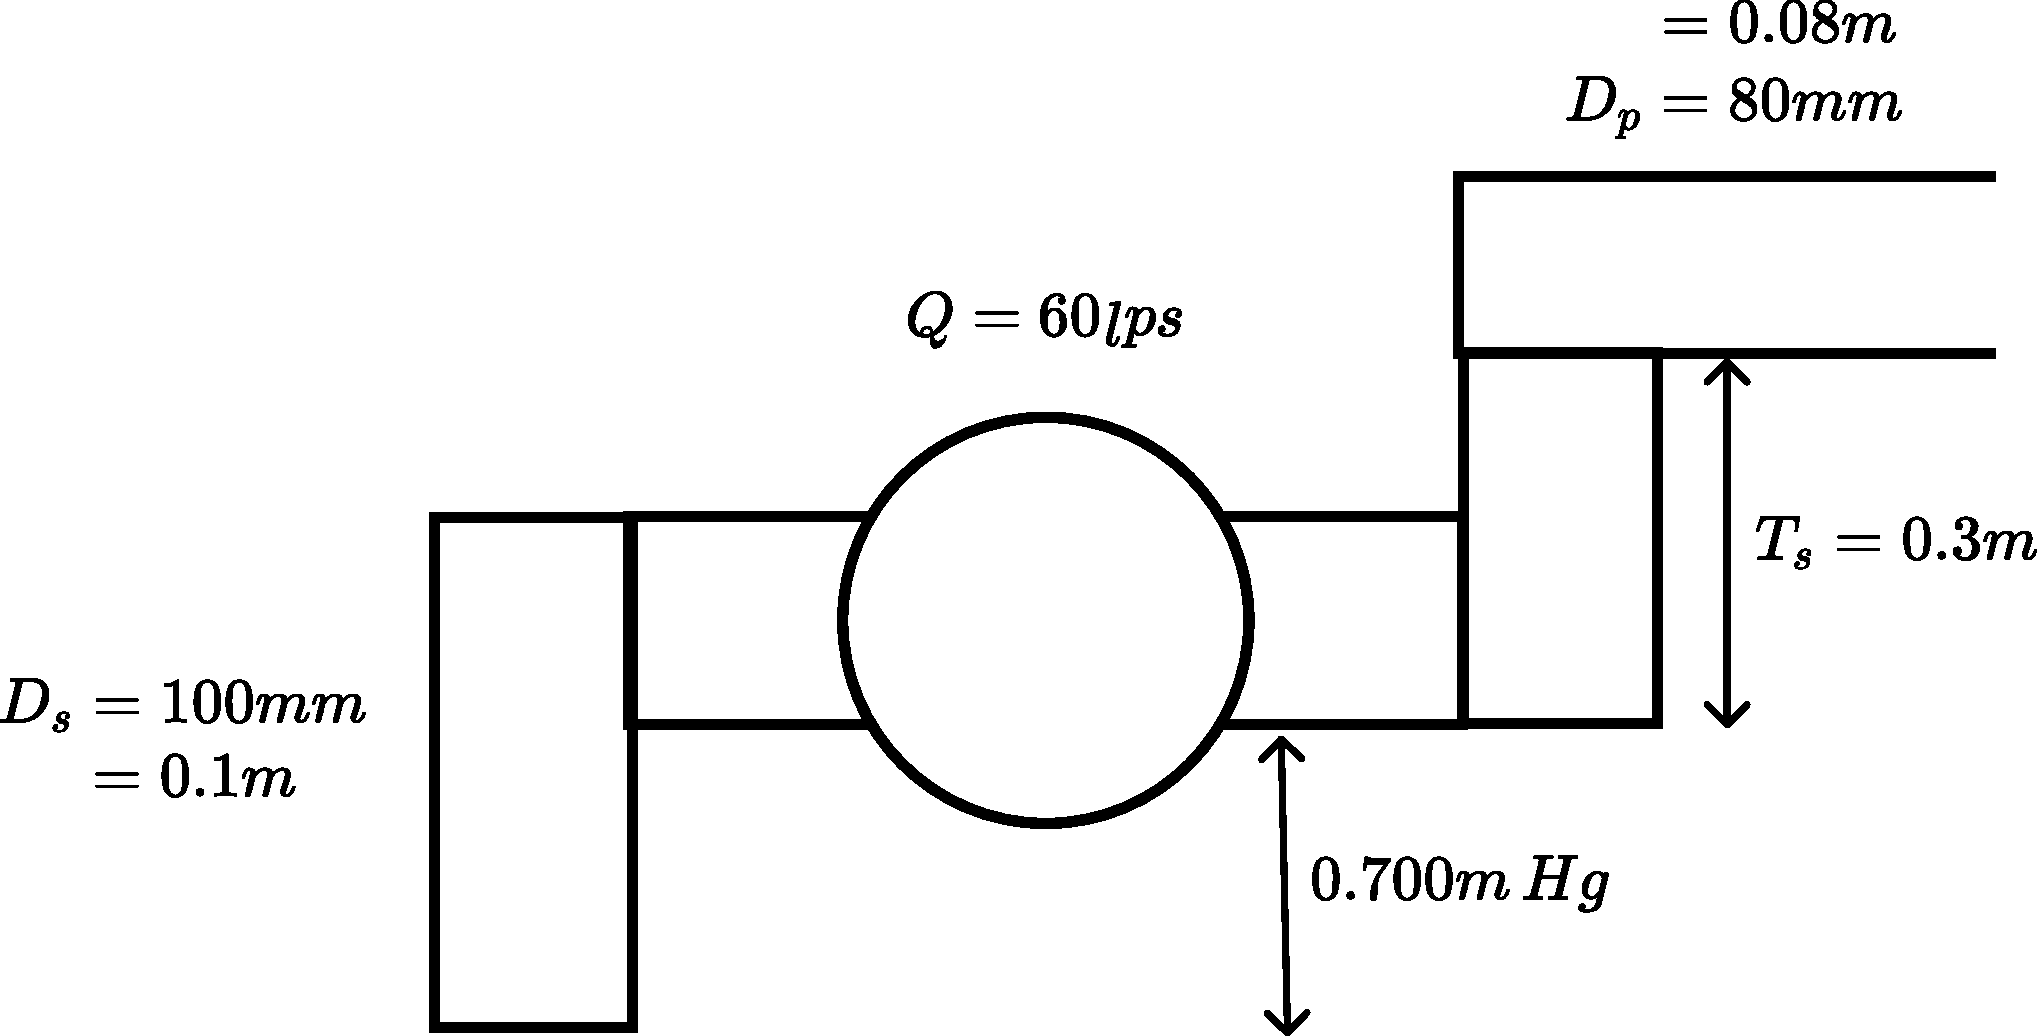
\includegraphics[width=0.5\textwidth]{eb7.pdf}
  \caption{Esquema del Problema}
  \label{eb7}
\end{figure}
\begin{align*}
    V_1 = \frac{Q}{A} = \frac{6011000}{\pi\cdot 100 / 1000^2 / 4} = 7.639 \frac{m}{s}\\
    V_2= V_1\left(\frac{D^2_1}{D^2_2}\right) = 7.639\left(\frac{100^2}{80^2}\right) = 11.94 \frac{m}{s}
\end{align*}
La ecuación general de la energía para el rendimiento  es:
\begin{align*}
    \frac{P_1}{\gamma} + \frac{V^2_1}{2g} + Hp = \frac{P_2}{\gamma} + \frac{V^2_2}{2g} + H\\
    H = \frac{\Delta P }{\gamma} + \frac{V^2_1 - V^2_2}{2g} + Hp
\end{align*}
La ecuación del rendimiento  del manómetro de mercurio es:
\begin{align*}
    &\frac{\Delta P}{\gamma} = R^{\prime}\left(5.9 - 1\right)H = \frac{700}{1000} \left(13.6 - 1 \right) - \frac{30}{100}\\
    &\frac{\Delta P}{\gamma} = 5.52\\
    &Hp = 5.52\frac{\left(11.95^2 - 7.639^2 \right)}{2*9.81} + \frac{30}{100} = 13.13Hp
\end{align*}


\subsection{Eficiencia electromecánica en equipos de bombeo para riego}
Evitar desperdicios y mejorar con técnicas modernas el riego en la agricultura (77\% del agua dulce utilizada en México se usa en la agricultura (CONAGUA, 2015))

Mejorar las eficiencias electromecánicas de los pozos de agua para riego en operación y selección optima de acuíferos

Haciendo un diagnóstico de la infraestructura de riego y pozos:

Riego: Verificar y medir la eficiencia de aplicación de riego y su infraestructura proponiendo métodos de riego eficientes.

Pozos: Verificar su eficiencia y mantenimiento de los pozos y proponer su rehabilitación y/o reposición, evitar nuevos afloramientos de agua subterránea

Equipo Electromecánico: Verificar que el equipo de bombeo y sistema electromecánico trabajen en máxima eficiencia (EEP)

Sistema Electromecánico

\begin{center}
    \smartdiagramset{border color=none,
    set color list={blue!50!cyan,green!60!lime,orange!50!red,red!80!black},
    back arrow disabled=true}
    \smartdiagram[flow diagram:horizontal]{Potencia\\Suministrada, $\eta$ Motor, $\eta$\\Transmisión, $\eta$ Bomba, Potencia Hudráulica}
\end{center}
\begin{align}
    &EEP=\eta_{elec}= \nu_{motor}\times \eta_{transmision}\times \eta_{bomba}\\
    &EEP=\eta_{elec}= \text{Eficiencia electromecánica de pozos}
\end{align}

Mediciones hidráulicas:
\begin{itemize}
    \item Medidor volumétrico
    \item Medidor ultrasónico
    \item Mediciones eléctricas con multiamperímetro y medidor de calidad de potencia
\end{itemize}

Cálculo de potencias

Hidráulica aprovechada
\begin{equation}
    P_a= \gamma QH
\end{equation}

Eléctrica consumida o suministrada:
\begin{equation}
    P_c = \frac{\sqrt{3} IT D}{746} 
\end{equation}
Cálculo de la eficiencia electromecánica
\begin{equation}
    H_{elec} = EEP= \frac{\text{Potencia aprovechada}}{\text{Potencia consumida}} \cdot  100
\end{equation}

De la norma oficial mexicana NOM-006-ENER-1995

Eficiencia energética electromecánica en sistemas de bombeo para pozo profundo en operación. Límites y método de prueba

Acciones a tomar de acuerdo a la norma, eficiencia energética electromecánica en sistemas de bombeo para pozo cuando EEP menor a 40\%
\begin{enumerate}
    \item a?
    \item Requerimiento nuevo electromecánico del pozo profundo
\end{enumerate}

\section{Bomba Turbina Vertical, Bomba de Flujo Mixto y Axial}










\subsection{Descripción, funcionamiento, ventajas y desventajas de las bombas centrífugas de paso múltiple}

\subsection{Trabajo realizado y eficiencia de la bomba}















































